\chapter{Fundamentação teórica}
\label{cap:fundamentacao}

\section{Ordenação de mensagens}
\label{sec:ordenacao_mensagens}

Um ordenador de mensagens é um mecanismo vital para promover coerência, em ordenação de eventos entre os participantes de um sistema distribuído e em um sistema replicado, usufruindo-se de replicação ativa, a ordenação de mensagens se torna vital para que o sistema evolua de maneira igual. Existem na literatura várias técnicas de ordenação de mensagens. A seguir são apresentados alguns tipos de ordenação de mensagens.

\subsection{Ordem FIFO}

A ordenação por \textit{First-In First-Out} (\gls{FIFO}), que significa o primeiro a entrar é o primeiro a sair, estabelece que as mensagens enviadas pelo mesmo participante e entregues para qualquer participante, são entregues na mesma ordem de envio \cite{PauloVerissimoLuisRodrigues}.

\begin{figure}[htb!]
    \centering
    \caption{Servidores S1 e S2 enviando mensagens FIFO}
    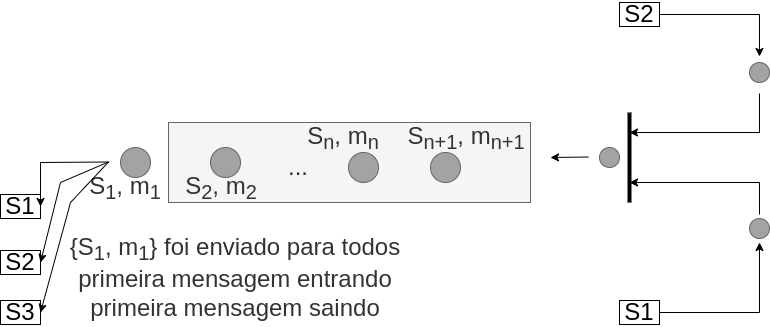
\includegraphics[width=0.8\linewidth]{figures/fifo.drawio.png}
    {\flushleft Fonte - Própria}
    \label{fig:fifo}
\end{figure}

A Figura \ref{fig:fifo} representa uma ideia de como o esquema de ordenação de mensagens FIFO pode funcionar. A ilustração em si demonstra que existe uma fila, que deve ser implementada por um ordenador de mensagens, assim as mensagens podem ser enfileiradas, ao passo que são enfileiradas, as mensagens também são consumidas na saída, dando vazão para as mensagens.

%\textbf{Causal}
\subsection{Ordem Causal}

A ordem causal, definida por Lamport \cite{lamport1978time}, estabelece algumas premissas: O símbolo $m$ é uma mensagem qualquer que acompanha um ID único e ${m_1, m_2, \dots, m_n} \in M$, onde M é um universo de mensagens; $send(m)$ é uma primitiva que executa o envio da mensagem $m \in M$; $p, q, r \in {participantes}$ onde os participantes são as entidades do sistema, que podem trocar mensagens entre si; $deliver(m)$ é uma primitiva de entrega de mensagens.

Na ordem causal, existe a definição da propriedade \textit{acontece antes}, simbolizado por $\longrightarrow$ e é um operador que designa uma ordem de precedência entre as mensagens.

Por ordem lógica, define-se: Uma mensagem $m_1$ precede logicamente $m_2$ \textit{i.e.} $m_1 \longrightarrow m_2$, sse: $m_1$ é enviada antes de $m_2$ pelo mesmo participante \textbf{ou} $m_1$ é entregue para o \textit{enviador} de $m_2$ antes que ele envie $m_2$ \textbf{ou} existe um $m_3$ tal que $m_1$ $\longrightarrow$ $m_3$ e $m_3$ $\longrightarrow$ $m_2$ \cite{PauloVerissimoLuisRodrigues}.
% Além disso,
%segue um paradigma lógico e é definida por \textcite{PauloVerissimoLuisRodrigues} como: ``

\textit{Exemplificando:} Se um evento $a$ aconteceu antes do evento $b$ \textit{i.e.} $a$ $\longrightarrow$ $b$, então o evento $b$ pode ter sido causado ou influenciado pelo evento $a$. Se $a$ e $b$ são duas mensagens \textit{multicast} (respeitando a causalidade), tem-se que a entrega de $a$ deve preceder a entrega de $b$, em todos os destinos comuns de $a$ e $b$. Abaixo está a especificação de entrega de pedido causal em grupos sobrepostos \cite{de1995causal}.

\begin{quote}
\textit{Definição de Ordem Causal}:\\
$send_p(m_1) \longrightarrow send_q(m_2)$
então
\\
$deliver_r(m_1) \longrightarrow deliver_r(m_2)$, \textit{i.e.} $m_1$
\\
é entregue para $r$ antes de $m_2$
\end{quote}

% Resumidamente, para quaisquer 
%2
% mensagens $m_1$ e, $m_2$ enviadas por $p$, respondidas por $q$, para o mesmo participante destinatário $r$, se $send_p(m_1) \longrightarrow send_q(m_2)$ então $deliver_r(m_1) \longrightarrow deliver_r(m_2)$, \textit{i.e.} $m_1$ é entregue para $r$ antes de $m_2$.
%'' 
A ordem causal pode ser implementada usando relógios lógicos de Lamport \cite{lamport1978time}
%, 
para capturar o sentido de causalidade sobre as entregas de mensagens.
%, entre os participantes. 
%A ordem causal permite eventos concorrentes acontecerem sem ordenamento, permitindo que computação paralela progrida sem restrições desnecessárias, mas em alguns casos é vital para o sistema que os eventos sejam ordenados \cite{PauloVerissimoLuisRodrigues}.

% Causal order lets concurrent events happen without ordering them. This is usually a positive feature, because it allows parallel computations to progress without unnecessary constraints.

\begin{figure}[htb!]
\centering
\caption{Exemplos de ordem causal}
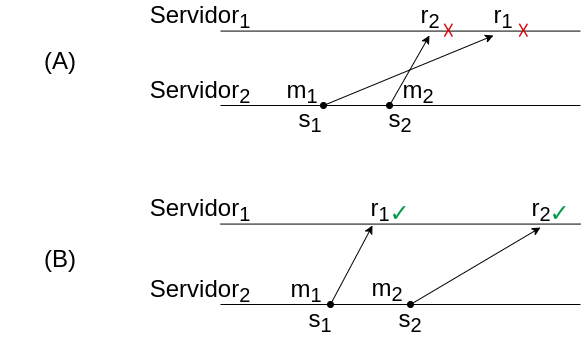
\includegraphics[width=0.8\linewidth]{figures/causal-order-works.drawio.png}
{\flushleft Fonte - Adaptado de \textcite{PauloVerissimoLuisRodrigues}}
\label{fig:causal-order-works}
\end{figure}

A Figura \ref{fig:causal-order-works} mostra dois exemplos (A e B) de ordem causal, os símbolos podem ser lidos da seguinte forma: $m_1$ e $m_2$ são mensagens, $s_1$ e $s_2$ são envios das mensagens, $r_1$ e $r_2$ são recebimentos das mensagens, $Servidor_1$ e $Servidor_2$ são os servidores do sistema distribuído. O exemplo (A) viola a ordem causal pois a mensagem $m_2$ chegou antes de $m_1$, sendo que $Servidor_2$ enviou primeiro $m_1$ e depois enviou $m_2$, ou seja, $m_1$ deve acontecer antes de $m_2$, pois existe uma relação de causa e ordem que deve ser obedecida. Essa relação pode ser observada no exemplo (B).

\subsection{Ordem Total}

Na ordenação total todos os participantes recebem as mensagens enviadas na mesma ordem. Porém, em termos mais técnicos, pode-se definir a partir de \textcite{PauloVerissimoLuisRodrigues} que:

\begin{quote}
\textit{Quaisquer duas mensagens entregues para quaisquer dois pares de participantes são entregues na mesma ordem para ambos os participantes.}
\end{quote}

O termo difusão em ordem total é também conhecido como difusão atômica, algumas vezes representado pela sigla \gls{AB-cast}. A seguir são apresentada as propriedades necessárias para assegurar ordenação total e os algoritmos para implementação de protocolo AB-cast.

% \begin{figure}[htb!]
%     \centering
%     \caption{Ilustração da ordenação total}
%     \includegraphics{figures/ordenacao-total.png}
%     \label{fig:total-ordering}
%     {\flushleft Fonte - Adaptado de \cite{journals/csur/DefagoSU04}}
% \end{figure}

% A Figura \ref{fig:total-ordering} ilustra o funcionamento da ordenação total, é possível observar que todas as mensagens que chegam, são difundidas de forma total e na mesma ordem de chegada.

%\subsection{Protocolos para Implementação de Ordem Total}
\section{Protocolos para Implementação de Ordem Total}

Define-se o problema com basicamente 2 primitivas e o conceito de processos corretos. As primitivas são \textit{TO-broadcast(m)} e \textit{TO-deliver(m)}, onde $m \in M$ é alguma mensagem que pode ser unicamente identificada e, que carrega a identificação do remetente, denotada por \textit{sender(m)} \cite{PauloVerissimoLuisRodrigues}.

A primitiva \textit{TO-broadcast} expressa a execução de difusão de uma mensagem para todos os processos corretos de um sistema, ou seja, todos esses processos corretos recebem as mesmas mensagens e na mesma ordem. \textit{TO-deliver} é outra primitiva que é executada sempre após \textit{TO-broadcast} \cite{PauloVerissimoLuisRodrigues}.

Os processos corretos pertencem a uma categoria de processos que não falham no sistema. Por exemplo, são processos que não omitem ou param de performar suas atividades de envio e recebimento de mensagens.
%, que respondem no tempo certo (exceto em sistemas assíncronos) e, que toleram falhas Bizantinas \cite{PauloVerissimoLuisRodrigues}. 
% A seguir é explanado alguns algoritmos que implementam \textit{TO-broadcast(m)}.

% qualquer outro algoritmo de consenso que utiliza ordem total como forma principal método de ordenação de mensagens.

A especificação básica para ordenação total,
conforme descrito por
%foi proposta por
\textcite{hadzilacos-10.5555/866693},
é apresentada a seguir:
%seguinte forma:

% \cite{journals/csur/DefagoSU04}
% (VALIDITY) If a correct process TO-
% broadcasts a message m, then it
% eventually TO-delivers m.

% (UNIFORM AGREEMENT) If a process TO-
% delivers a message m, then all correct
% processes eventually TO-deliver m.

% (UNIFORM INTEGRITY) For any message m,
% every process TO-delivers m at most
% once, and only if m was previously TO-
% broadcast by sender(m).

% (UNIFORM TOTAL ORDER) If processes p and
% q both TO-deliver messages m and m',
% then p TO-delivers m before m', if and
% only if q TO-delivers m before m'.

\begin{itemize}
\item \textbf{Validade}: Se um processo correto executa \textit{TO-broadcast} sobre uma mensagem $m$, então vai eventualmente executar \textit{TO-deliver} para a mensagem $m$.
\item \textbf{Acordo Uniforme}: Se um processo executa \textit{TO-deliver} sobre uma mensagem $m$, então todos os processos corretos irão eventualmente executar \textit{TO-deliver} sobre $m$.
\item \textbf{Integridade Uniforme}: Para qualquer mensagem $m$, cada processo executa \textit{TO-deliver} sobre uma mensagem $m$, pelo menos 1 vez, e apenas se previamente fora executado \textit{TO-broadcast} sobre uma mensagem $m$ por \textit{sender(m)}.
\item \textbf{Ordem Total Uniforme}: Se ambos os processos $p$ e $q$ executarem \textit{TO-deliver} sobre a mensagens $m$ e $m^{'}$, então $p$ executa \textit{TO-deliver} sobre $m$ antes de $m^{'}$, sse $q$ executa \textit{TO-deliver} sobre $m$ antes de $m^{'}$.
\end{itemize}

\subsection{Ordenação por sequenciador}

O algoritmo de ordenação por sequenciador \cite{journals/csur/DefagoSU04} tem a incumbência de ordenar todas as mensagens, sendo que para cada mensagem é associado um número de sequência. O algoritmo tem 3 papéis: o remetente (Algoritmo \ref{algo:simple-fixed-sequencer-sender}), o sequenciador (Algoritmo \ref{algo:simple-fixed-sequencer}) e os destinatários (Algoritmo \ref{algo:simple-fixed-sequencer-destinations}).

% \begin{enumerate}
% \item Todos os emissores enviam suas mensagens para o sequenciador.
% \item O sequenciador atribui um número de sequência único a cada mensagem.
% \item O sequenciador retransmite para todos os destinatários, usando ordem total.
% \end{enumerate}

%Logo a seguir expomos o algoritmo sequenciador fixo e, simples.

% \odo{O Algoritmo \ref{algo:simple-fixed-dest} apresenta .... } \ct{Indicar explicitamente e dizer o que cada algoritmo apresenta.}

% \textbf{Remetente}
% \begin{itemize}
% \item Executa a primitiva \textit{TO-broadcast(m)}, enviando \textit{send(m)} para o sequenciador.
% \end{itemize}

% \textbf{Sequenciador}
% \begin{itemize}
% \item Inicializa-se o número de sequência em 1.
% \item Quando o sequenciador recebe uma mensagem $m$
% \item O número de envio é inicializado com o valor de número de sequencia.
% \item Após isso, executa-se \textit{send(m, número de envio)} para todos os destinatários.
% \item Incrementa-se o número de sequência.
% \end{itemize}

% \textbf{Destinatários}
% \begin{itemize}
% \item Inicializa-se o número de próxima entrega em 1, e o conjunto de pendentes como vazio.
% \item Quando um processo destinatário recebe uma mensagem m com um número de sequência único.
% \item A mensagem m e, o número de sequência é unido ao conjunto de pendentes.
% \item Após unir as mensagens pendentes, executa-se um laço que percorre todas as mensagens que existem no conjunto de mensagens pendentes. Para cada $m$ que pertence ao conjunto de mensagens pendentes, executa-se \textit{entregar(m)}, ao final, incrementa-se o contador de próxima entrega.
% \end{itemize}

\begin{algorithm}
\DontPrintSemicolon
\procedure{TO-broadcast(m)} {
    send(m) to sequencer
}
\caption{Código dos remetentes para o algoritmo de sequenciador fixo simples}
\label{algo:simple-fixed-sequencer-sender}
\end{algorithm}


O Algoritmo \ref{algo:simple-fixed-sequencer-sender} apresenta a chamada do procedimento TO-broadcast(m). A primitiva TO-broadcast(m) é a representação da difusão por ordem total. Dentro do escopo do procedimento se executa a primitiva \textit{send(m)} ao sequenciador, discutido a seguir.

\begin{algorithm}
\DontPrintSemicolon

$seqnum := 1$

\when{receive(m)} {
    $sn(m) := seqnum$

    send(m, sn(m)) to all

    $seqnum := seqnum + 1$
}

\caption{Código do sequenciador para o algoritmo de sequenciador fixo simples}
\label{algo:simple-fixed-sequencer}
\end{algorithm}


O Algoritmo \ref{algo:simple-fixed-sequencer} representa o tratamento constante que é dado para mensagens $m$ que estão sendo recebidas. Começa com o número de sequência que recebe valor 1, esse valor é configurado uma vez apenas. Depois disto, o algoritmo só trata quando a mensagem $m$ existe e é recebida pela primitiva \textit{receive}.
O escopo de \textit{when receive(m)} tem 3 atribuições: na linha 3 o número de sequência de $m$ recebe o valor de \textit{seqnum} atual; na linha acontece o envio da mensagem $m$ junto com seu número de sequência através da primitiva \textit{send(m, sn(m))} para todos os participantes; na linha 5 ocorre o incremente do número de sequência.

\begin{algorithm}
\DontPrintSemicolon
\KwIn{Código do processo $p_i$}

${{nextdeliver}_p}_{i} := 1$\;
${{pending}_p}_{i} := \emptyset$\;

\when { receive (m, seqnum) } {
  ${{pending}_p}_{i} := {{pending}_p}_{i} \cup \{(m, seqnum)\}$\;
  \while { $\exists ({m}^{\prime}, {seqnum}^{\prime}) \in {{pending}_p}_{i}$ s.t. $seqnum^\prime = {{nextdeliver}_{p}}_{i}$} {
    \text{deliver}(${m}^{\prime}$)\;
    ${{nextdeliver}_p}_{i} := {{nextdeliver}_p}_{i} + 1$\;
  }
}
\caption{Código dos destinatários para o algoritmo de sequenciador fixo simples
\cite{journals/csur/DefagoSU04}}
\label{algo:simple-fixed-sequencer-destinations}
\end{algorithm}


O Algoritmo \ref{algo:simple-fixed-sequencer-destinations} inicializa os conjuntos de dados: \textit{nextdeliver} com todos os valores igual à 1, e \textit{ending} como vazio. Por conseguinte o algoritmo começa a processar continuamente o recebimento de mensagens, sendo que cada mensagem vem acompanhada de seu \textit{seqnum} (número de sequência). O primeiro passo dentro do escopo do \textit{when}, linha 4, implementa a união de novas mensagens no conjunto \textit{pending}. Quando o fluxo atinge a linha 5, ocorre um laço repetitivo. Neste laço repetitivo se verifica a existência de uma mensagem $m$ com \textit{seqnum} pertencente ao conjunto \textit{pending}, se for o caso então \textit{seqnum} receberá o valor de \textit{nextdeliver[$p_{i}$]} (final da linha 5). Após isso duas linhas de código são executadas, na linha 6 ocorre a execução da primitiva \textit{deliver(m)}. E na linha 7, ocorre o incremento de \textit{nextdeliver} na posição de $p_{i}$.


% \begin{comment}
% \odo{
% Exemplo de algoritmo. O Algoritmo \ref{alg:t} é apenas um exemplo de algoritmo em LaTeX, caso seja útil para você.

% \begin{algorithm}[!htb]

% %\caption{Transaction}\label{alg:t}
% \caption{T($cid,t$)}\label{alg:t}
% \begin{algorithmic}[1]
%   \State $ws \leftarrow \varnothing$; $rs \leftarrow \varnothing$; $i \leftarrow 0$;
%   \State choose randomly one of the replica servers $s$ \label{code:select_server}
%   %\ForAll {$t.getOp(i)$} \label{code:ws1}
%   \While {$t.getOp(i) \neq commit \wedge t.getOp(i) \neq abort$} \label{code:ws1}
%     \If {$t.getOp(i) = write$} \label{code:ws2}
%       \State $ws \leftarrow ws \cup (t.getItem(i),t.getValue(i))$
%     \EndIf
%     \If {$t.getOp(i) = read$}	
%       \If {$t.getItem(i) \in ws$}  \label{code:ws_copy1}
%         \State return $v$, s.t. $(t.getItem(i),v) \in ws$ \label{code:ws_copy2}
%       \Else
%         \State $c2s[s]!read,t.getItem(i),cid$  \label{code:read_request1}
%         \State $s2c[cid]?v,version$ from $s$  \label{code:read_request2}
%         \State $rs \leftarrow rs \cup (t.getItem(i),v,version)$ \label{code:read_request3}
%       \EndIf
%     \EndIf
%     \State $i$++;
%   \EndWhile
%   \If {$t.getOp(i) = commit$}   \label{code:if_commit}
%       \State $abcast.send(com\_req,cid,t.id,rs,ws)$    \label{code:abcast}
%       \State $s2c[cid]?outcome,s$	%\Comment{receive the $outcome$ from $s$}          
%       \State $t.result = outcome$ 
%   \Else \label{code:if_abort}
%       \State $t.result = abort$ 
%       %\State $return$ 
%   \EndIf

% \end{algorithmic}
% \end{algorithm}
% }
% \end{comment}

\subsection{Ordenação baseada em privilégio}

O algoritmo baseado em privilégio \cite{journals/csur/DefagoSU04} tem 2 papéis principais: os remetentes (Algoritmo \ref{algo:priviledge-based-simple-senders}) e os destinatários (Algoritmo \ref{algo:priviledge-based-simple-destinations}). A intenção geral do algoritmo é implementar a difusão atômica, para isso, rotaciona-se um \textit{token} entre os remetentes. Quando cada remetente recebe o \textit{token}, na sua vez, executa-se a primitiva \textit{tosend}, enviando para todos os destinatários as mesmas mensagens e na mesma ordem de chegada.
% Uma desvantagem do algoritmo baseado em privilégio é a dificuldade em atingir bons níveis de justiça (\textit{fairness}) entre todos os remetentes, a seguir exibimos o algoritmos remetentes e destinatários respectivamente.

% \textbf{Remetentes}

% \begin{itemize}
% \item Os enviadores são dispostos na forma de uma fila giratória (ou fila anelar).
% \item O primeiro da fila recebe o índice 0, e assim sucessivamente.
% \item A fila então deverá girar, porém quem começa operando é o $\text{sender}_0$.
% \item Quando a fila circula, o token deve ser passado ao próximo \textit{sender}.
% \item É atribuído para cada envio de mensagem um \textit{token} com número de sequência único.
% \item O procedimento de \textit{enviar} é basicamente \textit{TO-broadcast(m)}. Como já vimos, \textit{TO-broadcast(m)} é uma primitiva que faz a difusão ordem total das mensagens para os demais participantes do sistema.
% \item Quando um remetente recebe um \textit{token}, executa-se o seguinte: para cada destinatário \textit{send(m, número de sequencia do token)}, após isso, incrementa-se número de sequência do \textit{token}.
% \item Esse remetente passa o \textit{token} para o próximo da fila giratória.
% \item Como incrementamos o número de sequência do \textit{token}, não haverá colisão de número de sequências, e as mensagens poderão ser unicamente identificadas pelo seu número de sequência, no momento que o \textit{token} foi passado adiante.
% \end{itemize}

% \textbf{Destinatários}

% O algoritmo dos destinatários para o algoritmo baseado em privilégio é equivalente ao código para destinatários do algoritmo sequenciador fixo e simples.

\pagebreak

\begin{algorithm}
\DontPrintSemicolon
\KwIn{Código do processo $s_i$}

${{tosend}_s}_{i} := \emptyset$\;

\If {$s_i = s_1$} {
  token.seqnum := 1\;
  send token to $s_1$\;
}

\procedure { TO-broadcast(m) } {
  ${{tosend}_s}_{i} \cup \{m\}$\;
}

\when {receive token} {
  \foreach { ${m}{\prime}$ in ${{tosend}_s}_{i}$ } {
    send(${m}^{\prime}$, token.seqnum) to destinations\;
    $\text{token.seqnum} := \text{token.seqnum} + 1$\;
  }
  ${{tosend}_s}_{i} := \emptyset$\;
  send token to ${s}_{i+1 \mod n}$
}
\caption{Código dos remetentes para o algoritmo baseado em privilégios}
\label{algo:priviledge-based-simple-senders}
\end{algorithm}


O Algoritmo \ref{algo:priviledge-based-simple-senders} inicializa o conjunto \textit{tosend} como vazio. Se o processo $s_i$ é o primeiro, então inicializa \textit{token.seqnum} com 1 (linha 3) e, executa-se a primitiva \textit{send(token)} para $s_1$. Na linha 5 executa-se o procedimento de difusão ordem total sobre a mensagem $m$, na linha 6 a mensagem $m$ é unida ao conjunto \textit{tosend}. Na linha 7 quando o código dos remetentes recebe um novo token, executa-se, na linha 8, um laço iterativo, ou seja, para cada $m$ dentro do conjunto \textit{tosend}, executa-se, na linha 9, a primitiva \textit{send} para a mensagem $m$ junto com o valor atual de token.seqnum (rotacionando) para os destinatários. Na linha 10 a variável \textit{token.seqnum} recebe um incremento de 1. Fora do laço repetitivo, na linha 11, o conjunto \textit{tosend} recebe vazio. Na linha 12 executa-se a primitiva \textit{send} sobre o objeto \textit{token} para o processo $s$ porém é feito um cálculo modular para iterar pelos processos participantes de forma anelar. Uma vez que o próximo processo obtêm o \textit{token}, é a vez do processo recebedor de executar o algoritmo.

\begin{algorithm}
\DontPrintSemicolon
\KwIn{Código do processo $p_i$}

${{nextdeliver}_p}_{i} := 1$\;
${{pending}_p}_{i} := \emptyset$\;

\when { receive (m, seqnum) } {
  ${{pending}_p}_{i} := {{pending}_p}_{i} \cup \{(m, seqnum)\}$\;
  \while { $\exists ({m}^{\prime}, {seqnum}^{\prime}) \in {{pending}_p}_{i}$ s.t. $seqnum^\prime = {{nextdeliver}_{p}}_{i}$} {
    \text{deliver} ${m}^{\prime}$\;
    ${{nextdeliver}_p}_{i} := {{nextdeliver}_p}_{i} + 1$\;
  }
}
\caption{Código dos destinatários para o algoritmo baseado em privilégios \cite{journals/csur/DefagoSU04}}
\label{algo:priviledge-based-simple-destinations}
\end{algorithm}


O Algoritmo \ref{algo:priviledge-based-simple-destinations} e o Algoritmo \ref{algo:simple-fixed-sequencer-destinations} são iguais e portanto têm as mesmas explicações.

\section{Consenso}
\label{sec:consenso}

Protocolos de consenso distribuído também podem ser utilizados para implementar entrega totalmente ordenada de requisições \cite{conf/dsn/EkwallS06, MilosevicHutleSchiper2011}. Esses protocolos surgem como uma boa alternativa, visto que a difusão atômica pode gerar uma quantidade muito grande de requisições. Segundo \textcite{lamport2001paxos}, os algoritmos de consenso precisam garantir 3 premissas básicas:

\begin{itemize}
\item \textbf{Não trivialidade}: Um valor é aprendido se e somente se tiver sido proposto e aceito pela maioria dos participantes.

\item \textbf{Estabilidade}: A cada rodada de aprendizagem, qualquer processo participante deve aprender no máximo um valor. Um valor aprendido não deve ser alterado posteriormente pois um valor aprendido será executado na aplicação.

\item \textbf{Consistência}: A cada rodada de aprendizagem, dois processos diferentes não devem aprender valores diferentes.
\end{itemize}

\subsection{Protocolos de Consenso}

Protocolos de consenso são centrais para a implementação de aplicações distribuídas tolerantes a falhas \cite{cason2017role}.
O problema de consenso surgiu da necessidade de múltiplos
%computadores que compartilham o estado do sistema, 
processos chegarem a um acordo sobre um determinado valor. 
%Ou seja, para atingirmos harmonia entre os 
Portanto, participantes de um sistema distribuído
%de computadores precisamos de
necessitam de
um algoritmo capaz de estabelecer 
%um inquérito entre as máquinas. 
um quórum decisivo sobre um valor proposto pelo algoritmo de consenso.
%Veja que até o momento não precisamos mencionar se existe um tipo de aplicação específica, pois esse consenso é algo anterior a isso e, que deve estabelecer um acordo sobre algum comando antes desse comando ser executado por uma determinada aplicação.

% A seguir são apresentados 
%duas tecnologias, 
% dois protocolos de consenso
% bastante conhecidos
%, 
% na literatura.
%e, que implementam consenso, tipicamente ambos tem a intenção de oferecer uma evolução gradual e baseada em máquina de estados, da replicação dos \textit{logs} internos que contêm comandos que irão alterar o estado interno de uma aplicação.

\subsubsection{Paxos}

O algoritmo Paxos foi desenvolvido por \textcite{lamport2001paxos} e geralmente se implementa Paxos entre um conjunto distribuído de computadores trocando mensagens de forma assíncrona. Por exemplo, um cliente envia um valor ao sistema e o protocolo Paxos é invocado para propor este valor aos participantes. Quando a maioria dos participantes que executam o Paxos concordarem sobre o valor proposto, então este valor será aprendido e entregue aos interessados neste valor, por exemplo, a um conjunto de réplicas. Existem 3 papéis no algoritmo Paxos:

\begin{itemize}
\item \textit{Proponente:} Recebe solicitações de valores externos e as propõem aos aceitadores. Cada proposta nova deve conter um número único identificador e maior que a proposta anterior.

\item \textit{Aceitadores:} Aceitam determinado valor proposto pelo proponente e informam ao proponente e aos aprendizes se algum valor foi aceito. Uma resposta de um aceitador representa um voto para uma proposta. 
\item \textit{Aprendizes:} Aprendem o resultado do consenso, se houver.
\end{itemize}

\begin{figure}[htb!]
\centering
\caption{Exemplo de troca de mensagens no protocolo Paxos}
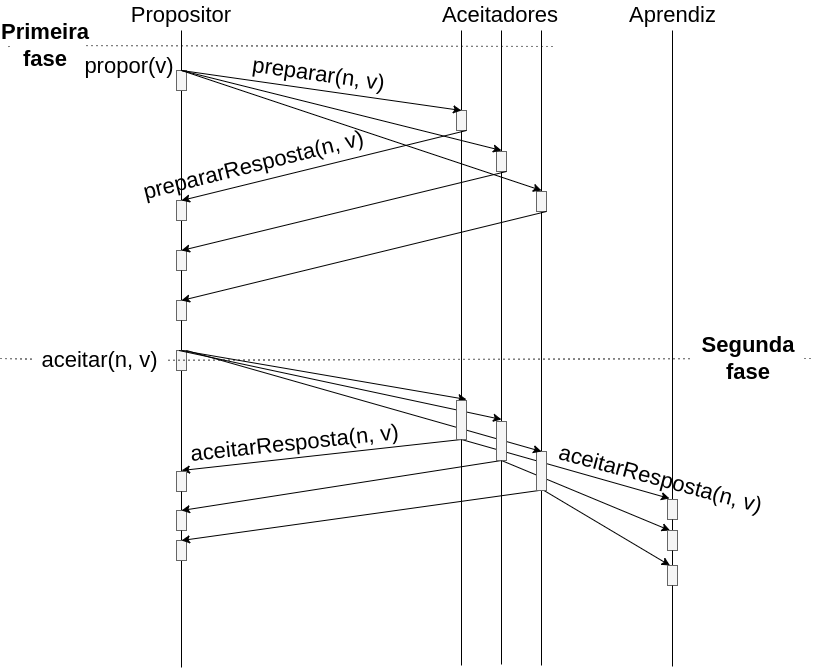
\includegraphics[width=1\linewidth]{figures/paxos.png}
{\flushleft Fonte - Adaptado de \textcite{AcaciaTerra}}
\label{fig:protocolo:paxos}
\end{figure}

O Paxos tem basicamente duas fases e a Figura \ref{fig:protocolo:paxos} ilustra as fases 1ª e 2ª. As fases foram subdivididas em a-b e que serão brevemente discutidas, a seguir.

\begin{enumerate}

\item \textit{Primeira fase: Proposta e Preparação}

\begin{enumerate}
\item O protocolo se inicia quando um proponente recebe um valor $v$. O valor $v$ pode ser, por exemplo, um comando que será executado em um determinado momento (no caso a natureza do valor $v$ depende muito da aplicação \textit{stateful}). O proponente propõe um valor $v$ enviando uma mensagem igual para cada um dos aceitadores. O algoritmo envia uma mensagem $v$ por proposta e está proposta terá outra difusão de mensagens para cada um dos aceitadores. Cada mensagem contém o valor da proposta e um número de sequência. O número de sequência é um identificador da proposta e quando o propositor propõe um valor $v$, este também prepara as mensagens e envia aos aceitadores.

\item Os aceitadores avaliam a proposta de valor e emitem suas respostas ao propositor, sinalizando que reconheceram a mensagem $m$ (que acompanha um número de sequência como identificador, juntamente com o valor proposto). Os aceitadores só devem aceitar a proposta com o número de sequência maior do que qualquer outro. A proposta já aceita com número identificador menor que o atual serão descartadas.
\end{enumerate}

\item \textit{Segunda fase: Aceitação e Aprendizado}

\begin{enumerate}

\item Os aceitadores recebem uma segunda rodada de mensagens,\\
onde o propositor
envia as mensagens, nesse estágio o propositor envia uma sequência de mensagens
para aceitar o valor $v$ com o número de sequência $n$, ou seja, os aceitadores 
recebem\\ \textit{aceitar(n, v)}.

\item O aprendiz aprende se os aceitadores chegaram a um consenso em uma rodada específica do algoritmo. A quantidade de aceitadores precisa ser pelo menos metade mais um, do conjunto de servidores do sistema. Se a maioria dos aceitadores responderem que concordam com o valor $v$, então $v$ será aprendido.
\end{enumerate}
\end{enumerate}

\pagebreak

\subsubsection{Raft}

O Raft é um algoritmo distribuído e assíncrono de ordenação de eventos \cite{raft}. Este algorítimo espera que exista um sistema de replicação de \textit{logs} em cada instância que executa o protocolo, e cada instância do sistema Raft pode estar em um dos seguintes estados: Líder, Candidato, Seguidor, porém só existe um líder por vez e o líder recebe requisições do cliente e pode propor mensagens aos seguidores.

\begin{figure}[htb!]
\centering
\caption{Fases de um serviço Raft}
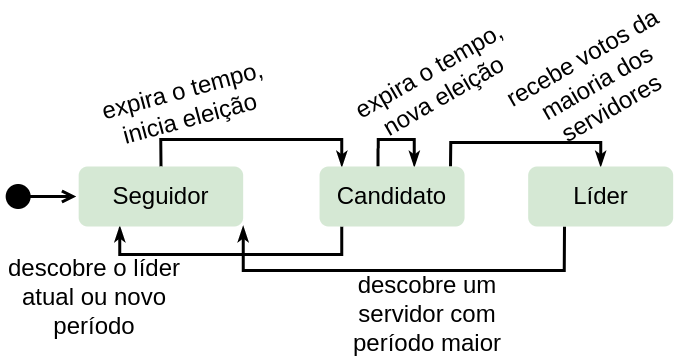
\includegraphics[width=0.75\linewidth]{figures/raft-states.drawio.png}
\label{fig:raft}
{\flushleft Fonte - Adaptado de \cite{raft}}
\end{figure}

A Figura \ref{fig:raft} ilustra os estados de cada nó participante e as possíveis transições. Os seguidores reagem às propostas do líder. Se os candidatos não recebem mais sinais do líder, elege-se um novo líder dentre os candidatos. Se algum candidato estiver no estado de seguidor, este deve poder votar por propostas que chegam ou votar para a eleição de novos líderes. É responsabilidade do líder fazer a replicação dos \textit{logs}. Deve haver apenas 1 líder por termo. O líder é responsável pela replicação de \textit{logs}.

\textcite{raft} buscaram desenvolver o algoritmo Raft com técnicas que aumentassem a legibilidade do algoritmo. Algumas das técnicas utilizadas foram: decomposição do problema em pequenas partes, minimização do espaço de estados, tratar múltiplos problemas com um único mecanismo, eliminação de casos especiais e minimização de não-determinismo.

% \item Os autores do Raft desenvolveram um mecanismo para decidir sobre informações obsoletas. Esse mecanismo se chama \textit{Term}.
% \item A ordem de prioridade dos termos aumentam de acordo com qual termo é mais recente. Os termos mais recentes são mais importantes. Existe então alguma noção de tempo inserida no algoritmo Raft.

\begin{figure}[htb!]
\centering
\caption{Termos em Raft}
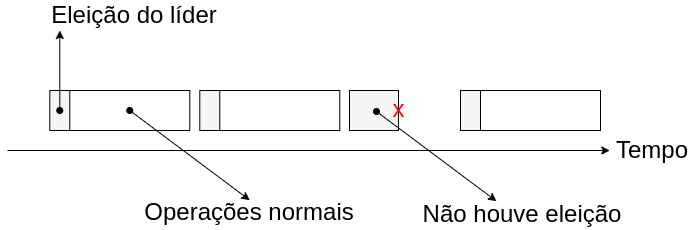
\includegraphics[width=0.8\linewidth]{figures/terms-raft.drawio.png}
{\flushleft Fonte - Adaptado de \textcite{raft}}
\label{fig:terms-raft}
\end{figure}

A Figura \ref{fig:terms-raft} ilustra um exemplo do funcionamento dos termos em Raft. Os \textit{Termos} em Raft existem para que o Raft possa identificar informação obsoleta e distinguir de informação nova. Cada máquina do \textit{cluster} mantêm o seu \textit{termo} atual e não são compartilhados globalmente. Cada \textit{Termo} se trata de um período de tempo onde ocorre uma eleição de um líder e após isso ocorrem proposta. Um \textit{Termo} é subdividido em 2 fases:

\textit{Primeira fase:} será feita a escolha de um líder.

\textit{Segunda fase:} serão feitas propostas de mensagens aos seguidores.

% Alguns \textit{Termos) podem não ter líder presente, quer dizer que houve falha na eleição.

% \subsubsection{Comparação entre Raft e Paxos}

% Em termos de provas formais, ambos buscam formalizar em provas matemáticas e premissas imutáveis, basicamente 4 regras formais dão embasamento formal. As regras formais são propriedades para atingir consenso assíncrono entre as partes envolvidas. A partir de estudos posteriores, os autores \textcite{MOSTEFAOUI_RAYNAL} esmiuçaram 4 regras formais e, que hoje estão elucidadas nas premissas a seguir:

% The Consensus Problem
% In the Consensus problem, every correct process Pi proposes a value v\ and all
% correct processes have to decide on the same value v, that has to be one of the
% proposed values. More precisely, the Consensus problem is defined by three safety
% properties (Validity, Integrity and Uniform Agreement) and a Termination Property
% [4,10]:
% [4] Chandra T. and Toueg S., Unreliable Failure Detectors for Reliable Distributed Systems. Journal of the ACM, 43(2):225-267, March 1996
% [10] Fischer M.J., Lynch N. and Paterson M.S., Impossibility of Distributed Consensus with One Faulty Process. Journal of the ACM, 32(2):374-382, April 1985
% • Validity: If a process decides v, then v was proposed by some process.
% • Integrity: A process decides at most once.
% • Uniform Agreement: No two processes decide differently.
% • Termination: Every correct process eventually decides on some value.

% \begin{enumerate}
% \item Validade: apenas os valores propostos podem ser decididos. Se um processo decidir sobre um valor, v, então algum processo precisa ter proposto v.
% \item Acordo uniforme: dois processos corretos (aqueles que não falham), não podem decidir sobre valores diferentes.
% \item Integridade: cada processo pode decidir 1 valor pelo menos 1 vez.
% \item Termo: todos os processos vão, eventualmente, decidir sobre um resultado.
% \end{enumerate}

% O Kubernetes, por padrão, não permite que StatefulSets obedeçam a terceira regra, Integridade. Apenas o nó mestre pode escrever na aplicação stateful, e se o nó mestre falhar outro nó deve ser eleito mestre, do contrário o cluster não irá mudar.

% Em termos de sistemas distribuídos, ambos servem casos de uso semelhantes, por exemplo: ``Quando múltiplas réplicas chegam à uma conclusão sobre um único comando?''. Paxos generalmente sacrifica disponibilidade \cite{cason2017role}, e o Raft opera as custas de disponibilidade. Quando nos deparados com particionamento de redes, Paxos vai continuar disponível, mas o \textit{cluster} Raft pode ficar parcialmente indisponível. Raft, e Paxos, são algoritmos de consenso que confiam na maioria do \textit{cluster}, em constante comunicação, para evoluir de estado. Em termos de didática, Raft tem um propósito de ser fácil de se compreender, enquanto Paxos não tem essa premissa. Ambos Paxos e Raft vão continuar operando enquanto o \textit{cluster} enfrenta falhas em seus nós.










% \section{Replicação por Máquinas de Estados}
% \label{sec:rep_maq_est}

% Implementar Replicação por Máquina de Estados (\gls{RME}) fornece tolerância a falhas. Também fornece escalabilidade, pois os clientes podem ler dados de qualquer servidor disponível
% \cite{lamport1978implementation, schneider1990}. 
% %O uso de Replicação por Máquina de Estados 
% %\odo{(\gls{RME})}
% %(RMS) 
% %foi proposto por \textcite{schneider1990} e, é comumente discutida na literatura o uso de RMS baseada em \textit{logs} \cite{lamport2001paxos}. 
% %Uma vantagem de usarmos máquina de estado é a promoção de tolerância a falhas e, o aumento da disponibilidade do sistema \cite{lamport1978implementation, schneider1990}. 
% De maneira geral, para a replicação por máquinas de estados funciona da seguinte forma: Configuramos um \textit{cluster} com várias máquinas replicando um mesmo serviço (\textit{i.e.} Banco de dados), e a medida que os clientes fazem suas requisições, a máquina de estados age como um replicador de \textit{logs}. Uma pré-condição para que todas as réplicas de máquina de estado se comportem de forma idêntica é executar as mesmas entradas de comando na mesma ordem. Os \textit{logs} aqui são as instruções que vão alterar dados da aplicação que o \textit{cluster} está servindo \cite{PauloVerissimoLuisRodrigues}. Os autores \cite{AlbuquerqueAlchieriCaetanoSolis2018} contribuíram com algumas especificações para Replicação por Máquina de Estados. A seguir será mostrado duas opções de modelagem, para manter serviços replicados:

% \begin{itemize}
% \item Apenas 1 mestre fixo que recebe todas as solicitações, e repassa essas solicitações para os demais participantes do sistema.
% \item Qualquer réplica pode se tornar um mestre eventualmente, através de um algoritmo de eleição.
% \end{itemize}

% Existem duas primitivas envolvidas em RME:

% \begin{enumerate}
% \item \textit{invoke(operation)}: essa primitiva é executada pelos clientes para chamar operações no serviço que implementa RME.
% \item \textit{execute(operation)}: essa primitiva é executada pelos servidores replicados, sempre que uma operação deve ser executada pelo serviço de RME.
% \end{enumerate}

% Além disso existem algumas propriedades para tornar o RME determinístico.

% \begin{itemize}
% \item Estado inicial: todas as réplicas corretas devem inciar a partir de um mesmo estado.
% \item Determinismo: todas as réplicas corretas, que executam uma mesma operação sobre um mesmo estado, realizam a mesma mudança em seus estados e produzem a mesma resposta.
% \item Coordenação: todas as réplicas corretas executam a mesma sequência de operações.
% \end{itemize}

% % \subsection{Replicação Ativa}

% % Difusão atômica é uma primitiva que tem influência quando se implementa replicação ativa \cite{lamport1978implementation, schneider1990}. A replicação ativa é uma técnica intuitiva que pode ser aplicada a máquinas de estado. Consiste em ter várias réplicas da mesma máquina de estado executadas por diferentes processos. Para garantir que o estado dessas réplicas seja mantido consistente, um protocolo de ordenação total deve ser usado para difundir os comandos da máquina de estado, no caso do \cite{PauloVerissimoLuisRodrigues}.

% A máquina de estados deve estar presente em cada réplica, e compartilhar um \textit{log} em comum e, a ideia é executar comandos do \textit{log}, igualmente em cada réplica, como é possível ver na Figura \ref{fig:rms}. Os comandos do \textit{logs} são comandos que foram autorizados por um algoritmo de consenso.

% \begin{figure}[htb!]
% \centering
% \caption{Eventos da Replicação por Máquinas de Estados}
% 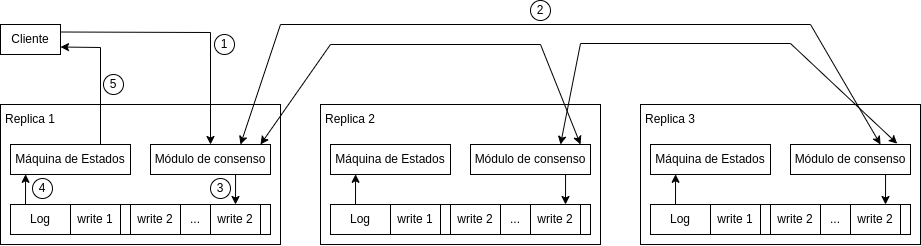
\includegraphics[width=1\linewidth]{figures/rms.drawio.png}
% {\flushleft Fonte - Adaptado de \textcite[p.~233]{journals/dbsk/SkrzypzcakS20}}
% \label{fig:rms}
% \end{figure}

% A Figura \ref{fig:rms} mostra que em um sistema distribuído essa máquina de estados deve ser replicada, ou seja, todos os servidores deste sistema distribuído deverão executar a mesma máquina de estados. Para fins de explicação, estamos considerando o módulo de consenso como uma caixa preta. As marcações numeradas na Figura \ref{fig:rms} são respectivamente:

% \begin{enumerate}
% \item Envia um comando qualquer para a Máquina de Estados Replicada.
% \item Entre em consenso sobre o comando.
% \item Concatena o novo comando.
% \item Aplica o comando que está na fila para ser executado, e que está no \textit{log}.
% \item Responde ao cliente.
% \end{enumerate}

% Cada nó, de um sistema distribuído, pode ser pensado como uma máquina de estados determinística. O intuito é prover tolerância a falhas, executando o mesmo registro de comandos, após cada ponto de salvamento. Idealmente essa é a ideia básica, porém na realidade existem  complicações, essas complicações motivam a pesquisa e desenvolvimento desse trabalho acadêmico. A imagem a seguir exemplifica, de maneira abstrata, como seria a replicação máquina de estados paralela. O desafio aqui é replicar o registro de comandos, igualmente, para todas as máquinas do sistema. Depois da replicação feita é necessário impor uma sincronização para que eles executem os comandos e a aplicação \textit{stateful} transite de estado, gerando um novo estado, porém são várias aplicações replicadas e iguais ao final do processo.










\section{Arquitetura de microsserviços}
\label{sec:arq_micro}

Publicações recentes mostram que implementar em arquiteturas de microsserviços provê desacoplamento e escalabilidade \cite{carrasco2018migrating, bavskarada2018architecting, zdun2019emerging}. O trabalho de \textcite{fritzsch2018monolith} provê dez abordagens estratégicas de refatoração, viabilizando migrar monólitos para microsserviços. A implementação de software seguindo arquitetura de microsserviços requer desenvolvimento de partes modulares, onde cada módulo pode ser conectado e desconectado em outros sistemas, sem que haja necessidade de mudar o sistema principal que faz uso do microsserviço. Geralmente, os microsserviços são enxutos com \textit{interfaces} específicas que viabilizam extensibilidade de funcionalidades específicas \cite{journals/software/JamshidiPMLT18}.

% não tenho citações pra isso
% Desenvolver arquitetura de microsserviços em Kubernetes tornou-se vigente, partindo do princípio de um \textit{cluster} servindo uma aplicação replicada. O \textit{cluster} Kubernetes permite que os desenvolvedores abstraiam a funcionalidade de um conjunto de \textit{Pods} e a exponham a outros desenvolvedores por meio de uma \gls{API}\footnote{API ou \textit{Application Programming Interface} é um conjunto de rotinas e padrões que facilitam a comunicação e troca de mensagens entre sistemas.}

% \subsection{Contêiner}

% A tecnologia de contêiner segue a característica de isolar várias tecnologias dentro de um pacote, os contêineres são diferentes de máquinas virtuais, por causa do advento em Linux de cgroups e namespaces, pois permitem que os contêineres usufruam diretamente dos recursos físicos, da máquina alvo.

\subsection{Contêineres e Orquestradores de contêineres}

% \textbf{O que é}

Um contêiner se trata de um ambiente empacotado de: software, configurações, dependências além de outras coisas para tornar possível que um serviço seja executado isoladamente de outros softwares da máquina hospedeira.

Um orquestrador é um gestor de contêineres com características de auto-cura e elasticidade. Também pode ser usado para a criação de \textit{cluster} (conjunto de máquinas interligadas por uma rede). Dependendo do fabricante da tecnologia algumas características podem mudar, porém geralmente o orquestrador tem características de: escalonamento de réplicas baseado em métricas, balanceamento de carga. Orquestradores podem operar sob os contêineres em grupos específicos \cite{casalicchio2019container}, descomplicando de se aplicar atribuições específicas para cada grupo de contêineres e podendo-se criar divisões lógicas que aprimoram a especificação do \textit{cluster} como um todo.

% \textbf{Contêineres}

\subsection{Docker}

Um contêiner Docker\footnote{\url{https://github.com/docker}} \cite{docker/docs/2022} é uma instância executável de uma imagem. Uma imagem do Docker é um modelo \textit{read only} que provê instruções para construção de um contêiner Docker. O Docker é uma tecnologia de código-aberto que oferece: preparo, entrega e execução de aplicativos auto-contidos em contêineres. Com Docker é possível: criar, iniciar, parar, mover e excluir um contêiner usando a \gls{API} do Docker. O Docker integra com funcionalidades Linux como \textit{cgroups} e \textit{namespaces} para usufruir dos recursos da máquina hospedeira, permitindo melhor desempenho. Além disso, existe uma extensa comunidade adepta ao Docker, que contribui com melhorias constantes ao Docker. 

% Existem várias alternativas ao Docker, alguns exemplos são: Podman, LXD, Containerd. Para este trabalho, optou-se pelo Docker pois existe uma documentação extensa e, muitos contribuidores, por exemplo desenvolvedores implementam soluções e as compartilham no DockerHub (uma central de implantações prontas). O Docker também é bastante aceito pela comunidade científica para aumento da reprodutibilidade \cite{CitoGallDockerReproducibility}. Além disso nem todas as tecnologias de contêiner são suportados pelo Kubernetes.

% \textbf{Por quê usamos Kubernetes}

% Segundo \textcite{soppelsa2016native} existem alternativas ao Kubernetes, por exemplo o Docker Swarm. Swarm é um modo nativo da tecnologia Docker, que permite orquestração dos contêineres, ou seja herda as características de auto-cura, balanceamento de carga, \textit{etc}. Kubernetes da suporte para Docker, Containerd, CRI-O e, qualquer outra tecnologia de contêiner que implementa a interface Kubernetes CRI (Container Runtime Interface) \cite{kubernetes/docs/2022}, e uma vantagem de usarmos Kubernetes é devido ao Kubernetes CRI. O Docker Swarm poderia ser usado no lugar de Kubernetes, porém estamos enxergando muito mais aderência ao Kubernetes do que outras alternativas, nas bases científicas, um dos motivos pode ser a influência da Google sob o Kubernetes, apesar de hoje em dia não ser mais um projeto Google, mas sim um projeto da \textit{Cloud Native Computing Foundation}. Esperamos saber responder como Kubernetes se comporta após ter sido incrementado com serviço de replicação por máquinas de estados e consenso, ou seja, quais são as vantagens e desvantagens.

\subsection{Kubernetes}

Kubernetes é uma ferramenta de orquestração de contêineres inicialmente desenvolvida por engenheiros da Google. Kubernetes providencia primitivas tais como: Nodes, Services, Pods, Deployment, Job, Secret, ReplicaSet, StatefulSet, Volume, dentre outras, para que desenvolvedores possam definir Clusters. Kubernetes resolve problemas de estabelecimento de rede entre as máquinas que compõe o Cluster, sejam elas físicas ou virtuais. Kubernetes também resolve problema de replicação de serviços, todavia não garante que os dados das réplicas serão replicados de maneira consistente \cite{kubernetes/docs/2022}. Quando se trata de sistemas com replicação, busca-se uma infraestrutura robusta que permite que cada réplica possa ter seus recursos garantidos \cite{Stubbs2015DistributedSO}, baseado em métricas e tolerante a falhas \cite{vayghan2021kubernetes}.

\subsubsection{Detalhes da tecnologia Kubernetes}

A disponibilidade do Kubernetes foi avaliada por \cite{vayghan2021kubernetes} e o Kubernetes provê mecanismos que operam para deixar o Cluster operacional e servindo. A escalabilidade e recuperação de desastres é algo que o Kubernetes prove automatizações pré-configuráveis. A escalabilidade permite expandir ou retrair a quantidade de nós de trabalho no \textit{cluster}, dependendo da carga sob demanda. A recuperação de desastres trata de prover a restauração de \textit{Pods} em casos de falhas. Dentre os vários tipos de componentes do Kubernetes se pode mencionar alguns básicos:

\textit{Nodes:} São máquinas físicas ou virtuais que têm como principal função executar os \textit{Pods}. Tipicamente um nó em Kubernetes é visto como um servidor. A infraestrutura do Kubernetes segue o esquema Líder-Seguidores, onde o nó líder opera sob os nós seguidores.

\textit{Services:} Um \textit{Service} define um conjunto de \textit{Pods} que provê serviços variados.

% Uma vez que o \textit{cluster} Kubernetes está configurado, será necessário o uso de um outro componente interno chamado Kubernetes DNS (\textit{Domain Name System}). O Kubernetes provê um serviço de DNS capaz de localizar os endereços dos \textit{Pods}, no \textit{cluster}. O DNS \textit{server} do \textit{cluster} Kubernetes é instalado no sistema quando o \textit{cluster} é criado no sistema operacional \textit{host}. A função do Kubernetes DNS é fornecer a localização em termos do IP de cada nó do \textit{cluster}.

% Kubernetes:Pod

\textit{Pod:} A menor unidade que o orquestrador administra, um \textit{Pod} pode conter múltiplos contêineres em execução, mas tipicamente cada \textit{Pod} contém apenas uma aplicação isolada em contêiner. \textit{Pod} são efêmeros, significa que podem encerrar seu ciclo de vida, se um \textit{Pod} morrer um novo \textit{Pod} será alocado no lugar. Cada \textit{Pod} recebe um endereço IP\footnote{IP: \textit{Internet Protocol} se trata de um endereço que identifica um dispositivo na rede.} mas se um \textit{Pod} morrer e for substituído por um novo, o endereço IP permanece o mesmo.

% Kubernetes:Kubectl

\textit{Kubectl:} É uma ferramenta de comandos em linha, para ser executado em um \textit{Terminal}. O Kubectl permite executar operações em Kubernetes, mas é preciso um arquivo \textit{YAML} que descreve tudo sobre o \textit{cluster} Kubernetes.

% Kubernetes:PersistentVolumes

\textit{PersistentVolumes:} Se trata de um componente que administra a persistência dos dados, podendo ser local ou remoto. O Kubernetes não faz backup dos dados, ficando a cargo do desenvolvedor implementa-lo. Os modos de acesso aos volumes persistentes são: leitura e escrita por um nó único (\gls{RWO}); somente leitura por vários nós (\gls{ROX}); leitura escrita por vários nós (\gls{RWX}).

% O \textit{Pod} com permissão de escrita dos dados é chamado de \textit{leader}, os demais \textit{pods} são chamados de \textit{followers}. Uma vez que novos dados foram escritos no banco, um outro mecanismo fará a sincronização dos dados, fazendo com que todos as aplicações \textit{stateful} evoluam igualmente. Para manter os dados preservados é necessário configurar \textit{PersistentVolume} para \textit{StatefulSet}, pois os ciclos de vida do \textit{PersistentVolume} e do \textit{StatefulSet} são desacoplados. Cada \textit{Pod} em modo \textit{StatefulSet} recebe um nome especial no formato de \textit{\$\{statefulset name\}-\$inteiro positivo começando de 0}. O Kubernetes não faz a clonagem, sincronização ou, o \textit{backup} dos dados, ficando a cargo do desenvolvedor configurar isso dentro do \textit{StatefulSet}.

% O \textit{Heartbeat} é um sinal que o nó seguidor emite para o nó mestre avisando qual o estado de saúde dos \textit{Pods}.

% O Kubernetes provê um componente de armazenamento chave-valor e não-volátil, chamado Etcd. O banco Etcd funciona como o cérebro do Kubernetes. O Etcd armazena dados de todos os nós, assim o Kubernetes pode executar ações de \textit{auto medicação}, ou \textit{auto escalonamento}, baseando-se nas informações sobre os estados de cada \textit{Pod} do \textit{cluster} Kubernetes.

% Kubernetes:{Kubelet, ApiServer, PodSpec, YAML}

\textit{Kubelet:} É um componente básico de cada um Nó do Kubernetes. O \textit{Kubelet} é requisitado pelo Kubernetes do nó controlador para receber informações sobre estatísticas de todos os nós do cluster, com essas essas informações o Kubernetes faz a gestão automática dos Nós e seus componentes internos.

% Kubernetes:ReplicaSet

\textit{ReplicaSet:} Mantêm as réplicas de um \textit{cluster} Kubernetes. É definido com os campos: seletor que especifica como identificar os \textit{Pods}, número de réplicas indicando quantos \textit{Pods}, e um \textit{template} do \textit{Pod} para poder replicar igualmente.

\textit{Deployment:} O Deployment define como criar e atualizar instâncias do seu aplicativo.

% Kubernetes:LoadBalancer

% Para podermos manter o balanceamento de carga do \textit{cluster}, Kubernetes provê um componente chamado \textit{LoadBalancer}, que direciona as requisições para réplicas. Métricas como quantidade de: UCP disponível, Memória Ram, Latência da rede, \textit{etc}., podem ser usadas para definir qual replica receberá a carga de trabalho.

% Balanceamento de carga funciona de forma diferente para aplicações Stateful

% Kubernetes:Secrets

% É importante também lembrar de manter em segredo algumas informações sensíveis. O Kubernetes \textit{Secrets} é outro componente do Kubernetes que guarda as informações sigilosas, da sua aplicação tais como senhas, \gls{API} \textit{tokens}, \textit{ids}, etc., sem que os desenvolvedores precisem ter isso no código da aplicação ou nos arquivos de configuração. É necessário que os dados sigilosos guardados no \textit{Secrets} estejam codificados em base64. No entanto o \textit{Secrets} não encripta os dados sigilosos, por padrão. O desenvolvedor precisa seguir alguns passos para ter os dados criptografados no \textit{Secrets}.

\textit{Jobs}: é um componente que pode criar um ou mais \textit{Pods}, e executará um procedimento até que os \textit{Jobs} possam terminar. O Kubernetes mantém o número de Jobs que estão finalizando com sucesso e, se esse número chegar até um valor especificado então o Kubernetes vai entender como missão bem sucedida.

% \begin{figure}[!htb]
% \centering
% \caption{Arquitetura do \textit{Cluster} Kubernetes}
% 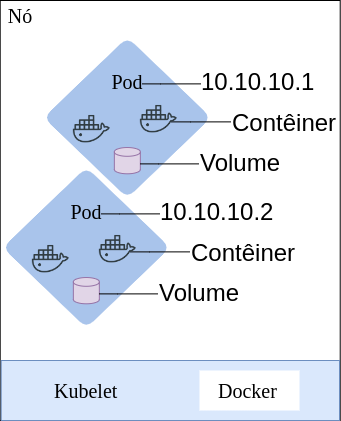
\includegraphics[width=0.4\linewidth]{figures/kubernetes-arch.png}
% {\flushleft Fonte - Adaptado de \textcite{renan2021hermes}}
% \label{fig:kubernetes-architecture}
% \end{figure}

% A Figura \ref{fig:kubernetes-architecture} representa uma forma de esquematizar um \textit{cluster} Kubernetes com o Hermes servindo à frente de uma aplicação \textit{stateful} alvo. O \textit{cluster} Kubernetes pode conter vários nós, cada nó tem 1 Kubelet e suporte para Docker contêineres, cada nó pode conter 1 ou mais \textit{Pods}, cada \textit{Pod} tem 2 imagens de contêineres (uma para o Hermes e outra para a aplicação \textit{stateful} alvo, cada \textit{Pod} tem seu IP na rede privada do Kubernetes e cada Pod contêm seu volume persistente. O padrão de projeto Sidecar, foi implementado junto ao Kubernetes, onde o contêiner do Hermes é lançado ao lado do contêiner da aplicação alvo.
